\documentclass{article}

% ============================================================
% MA 213 In-Class Worksheet Template
% Student-facing worksheet for lecture activities.
% ============================================================

\usepackage[margin=1in]{geometry}
\usepackage{amsmath}
\usepackage{xcolor}
\usepackage{parskip}
\usepackage{array}
\usepackage{enumitem}
\usepackage{booktabs}
\usepackage{graphicx}

\newcommand{\coursenumber}{MA 213}
\newcommand{\weekplaceholder}{11}
\newcommand{\lectureplaceholder}{27}
\newcommand{\lecturetitle}{Intuition for Power Changes: Think/Pair/Share}

\newcommand{\nameblank}{\rule{1.75in}{0.4pt}}
\newcommand{\idblank}{\rule{1.55in}{0.4pt}}
\newcommand{\shortblank}{\rule{1in}{0.4pt}}
\newcommand{\longblank}{\rule{0.93\linewidth}{0.4pt}}

\begin{document}

\begin{center}
  {\LARGE \coursenumber{} Week \weekplaceholder{}: Lecture \lectureplaceholder{}}\\
  {\large \lecturetitle{}}
\end{center}

\begin{enumerate}[label=\arabic*.,leftmargin=*,itemsep=.7em]
  \item \textbf{Your name:} \nameblank \hfill \textbf{BU ID:} \idblank
\end{enumerate}

\textbf{Big idea:} The figure below shows a baseline scenario for a two-sided test: the null distribution (blue, centered at 0) and the alternative distribution (green, centered at the true effect size, here 2.5), both with standard error $SE=1$. The dashed lines mark the rejection region boundaries for $\alpha = 0.05$, and the shaded green area is the power --- the probability of rejecting $H_0$ when this alternative is true.

\begin{center}
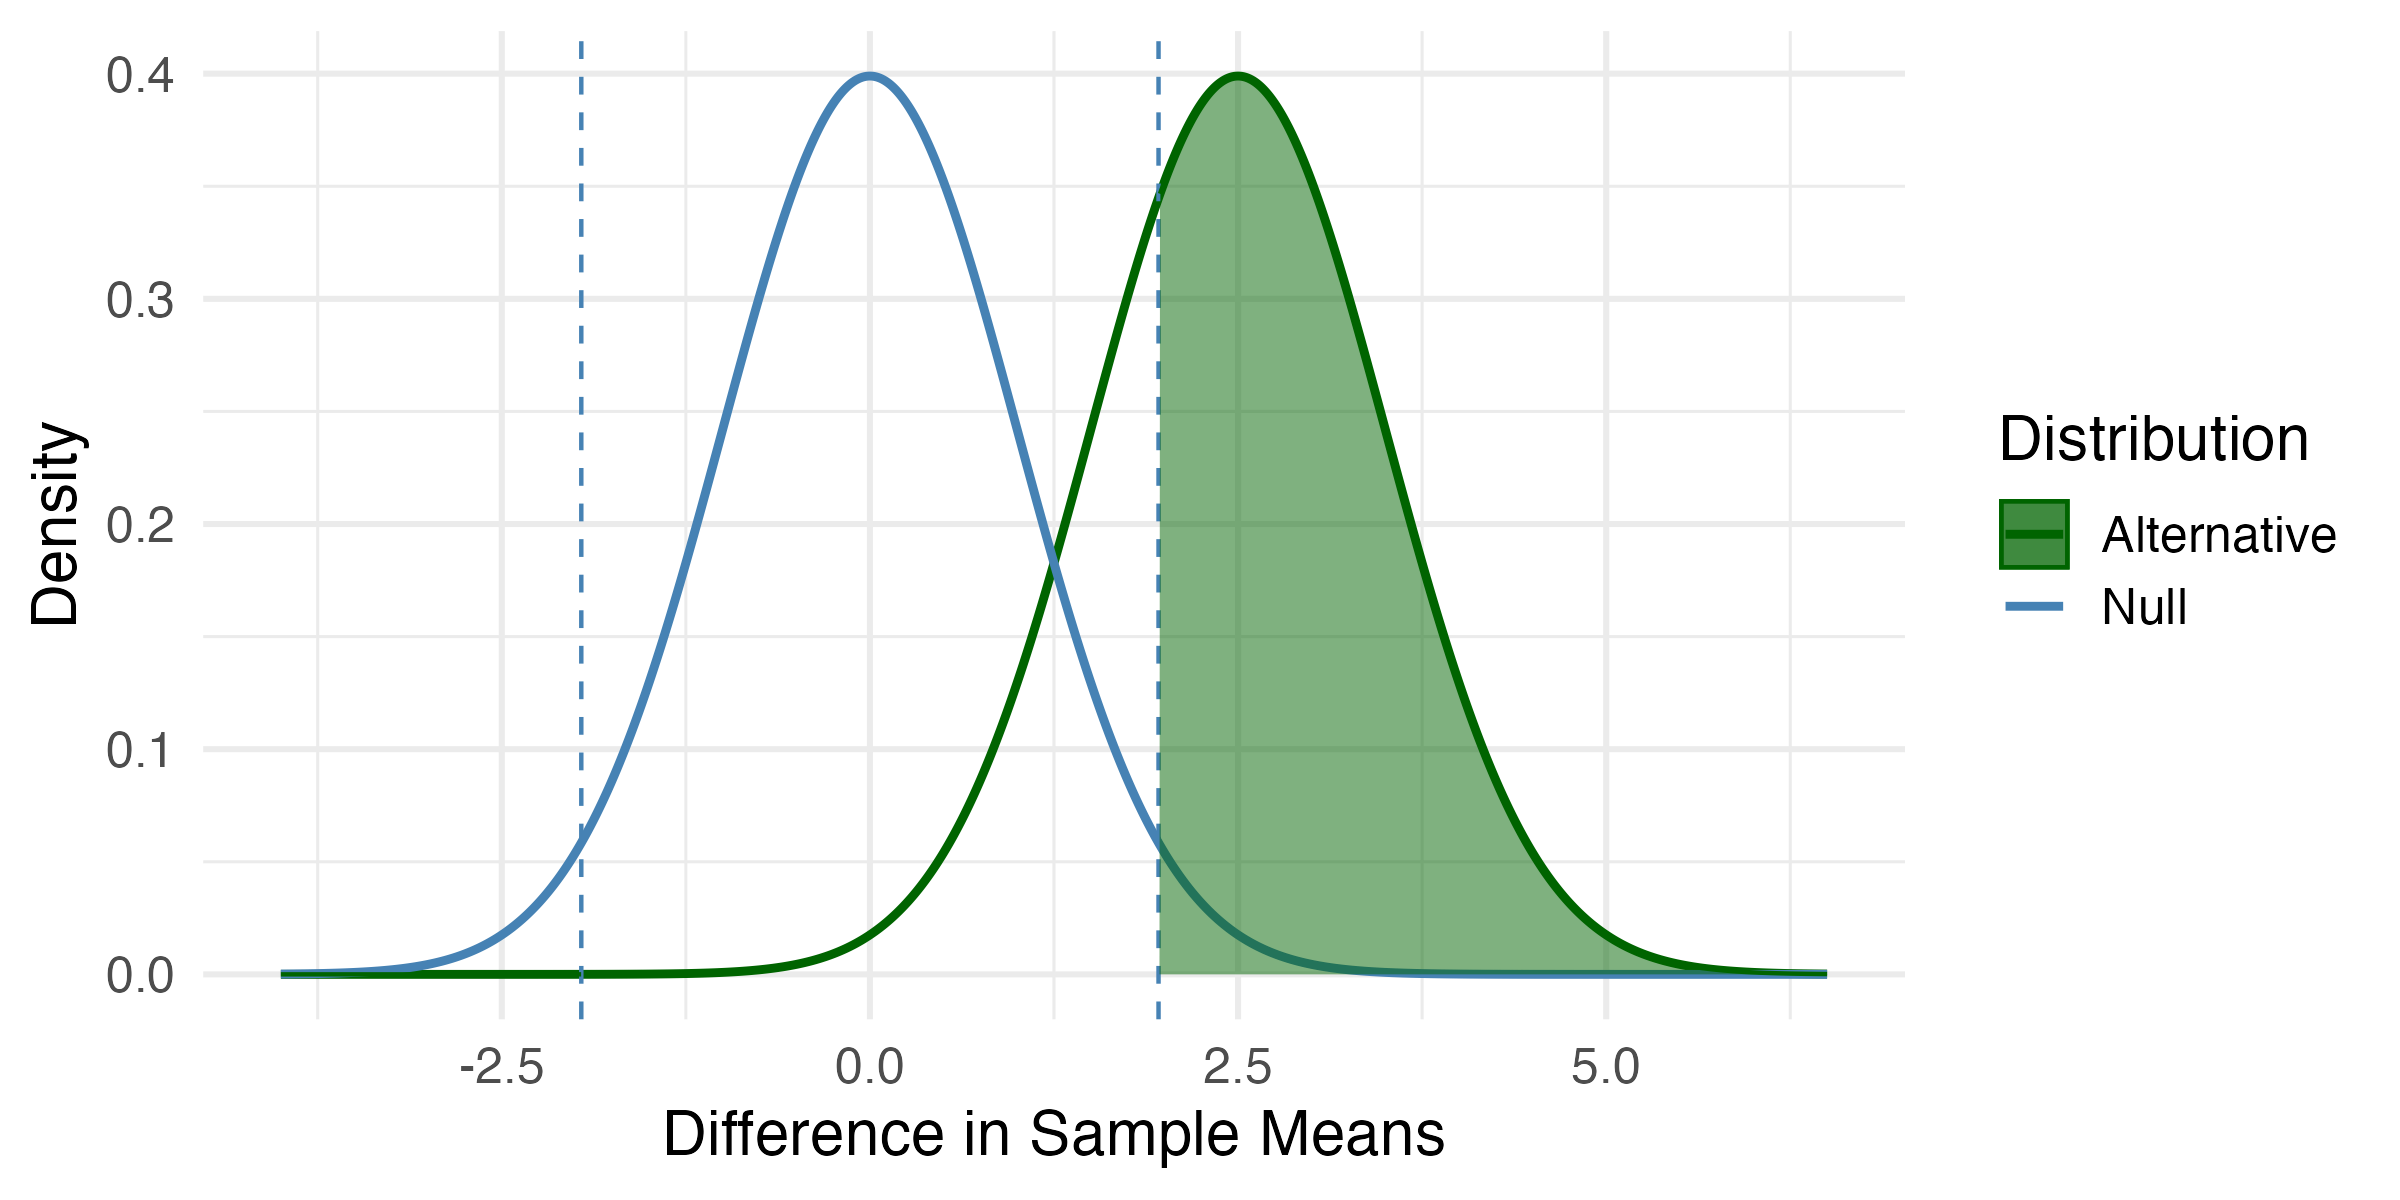
\includegraphics[width=0.75\textwidth]{figures/whatif_baseline.png}
\end{center}

\section*{Step 1: Think (2 mins)}
Hint: none of these questions require any calculations --- just think about how changing one quantity moves the curves or the dashed lines, and how that changes the shaded area. There are more hints on the next page if you get stuck.

\textbf{(a)} Starting from this baseline, what happens to the power if we \emph{increase the effect size} (move the alternative mean farther from 0)? Circle one, and explain why in a sentence.
\begin{center}
Increase \hspace{0.5in} Decrease \hspace{0.5in} Stay the same
\end{center}
\vspace{0.5in}

\textbf{(b)} What happens to the power if we \emph{decrease $\alpha$} (e.g.\ from 0.05 to 0.01)? Circle one, and explain why in a sentence.
\begin{center}
Increase \hspace{0.5in} Decrease \hspace{0.5in} Stay the same
\end{center}
\vspace{0.5in}

\textbf{(c)} What happens to the power if we \emph{increase the sample size} (which decreases $SE$)? Circle one, and explain why in a sentence.
\begin{center}
Increase \hspace{0.5in} Decrease \hspace{0.5in} Stay the same
\end{center}
\vspace{0.5in}

\newpage
\section*{Hints for Step 1}

\textbf{(a)} Increasing the effect size shifts the green (alternative) curve away from the blue (null) curve, without moving the dashed rejection-region lines. Does the green curve now overlap \emph{more} or \emph{less} with the region inside the dashed lines?

\vspace{0.2in}

\textbf{(b)} Decreasing $\alpha$ makes it harder to reject $H_0$ by requiring more extreme evidence, which pushes the dashed lines \emph{outward}, away from 0. The green curve doesn't move. Does the shaded area (outside the new, wider-spaced lines) get bigger or smaller?

\vspace{0.2in}

\textbf{(c)} Increasing the sample size shrinks $SE$, which makes \emph{both} curves narrower (more peaked) without moving their centers. What happens to the dashed lines? Sketch a quick picture --- does the green curve's area outside the lines grow or shrink?

\vspace{0.2in}
\noindent\rule{\linewidth}{0.4pt}
\vspace{0.2in}

\section*{Step 2: Pair (2 mins)}

\begin{enumerate}[label=\arabic*.,leftmargin=*,itemsep=.7em, start=2]
  \item \textbf{Partner's name:} \nameblank \hfill \textbf{BU ID:} \idblank
\end{enumerate}

Compare your answers with your partner. Then discuss:

\begin{itemize}
  \item Did you agree on all three? If not, sketch the curves together to settle the disagreement.
  \item Of the three levers (effect size, $\alpha$, sample size), which is usually easiest for a researcher to control in practice? Which is hardest?
\end{itemize}

\textbf{Our thoughts:}
\vfill

\end{document}
